\begin{figure}
    \centering
        \begin{subfigure}[b]{0.49\textwidth}
         \centering
         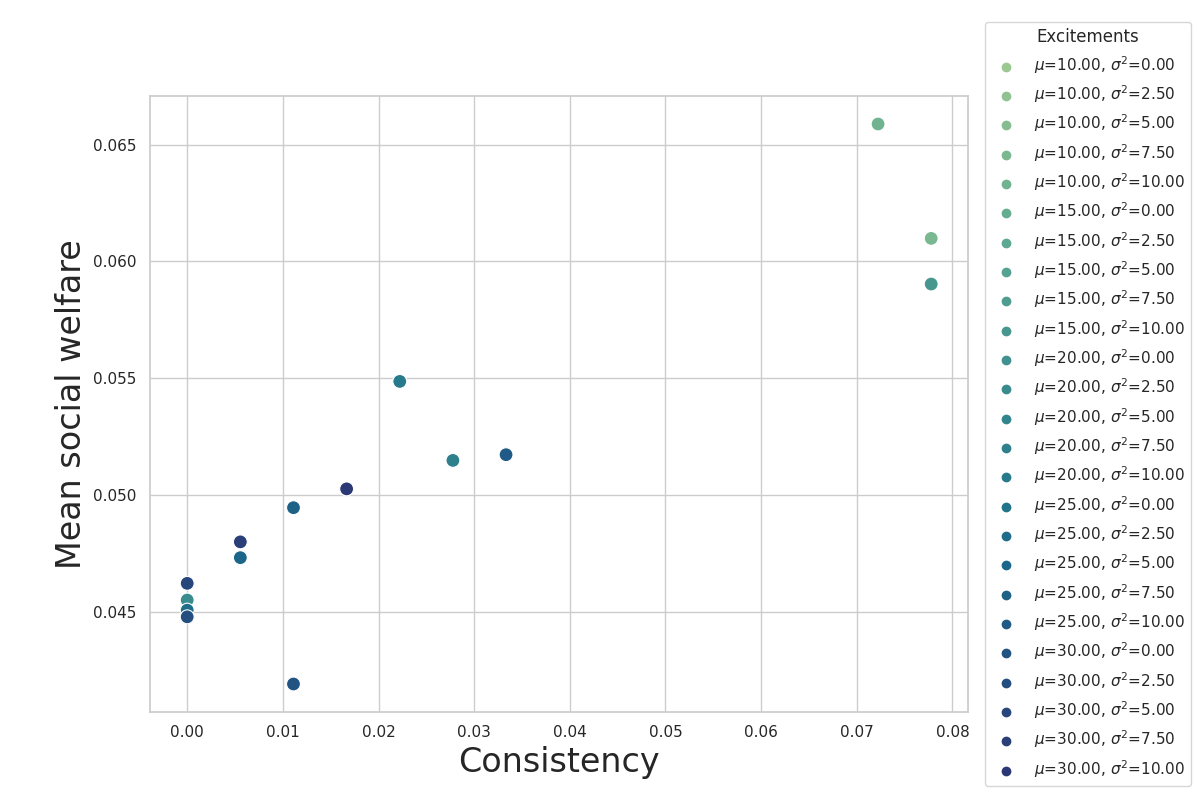
\includegraphics[width=\textwidth]{figures/mpda_dynamics_initliazation.png}
         \caption{Dynamic Initialization}
         \label{fig:init}
        \end{subfigure}
         \begin{subfigure}[b]{0.49\textwidth}
         \centering
         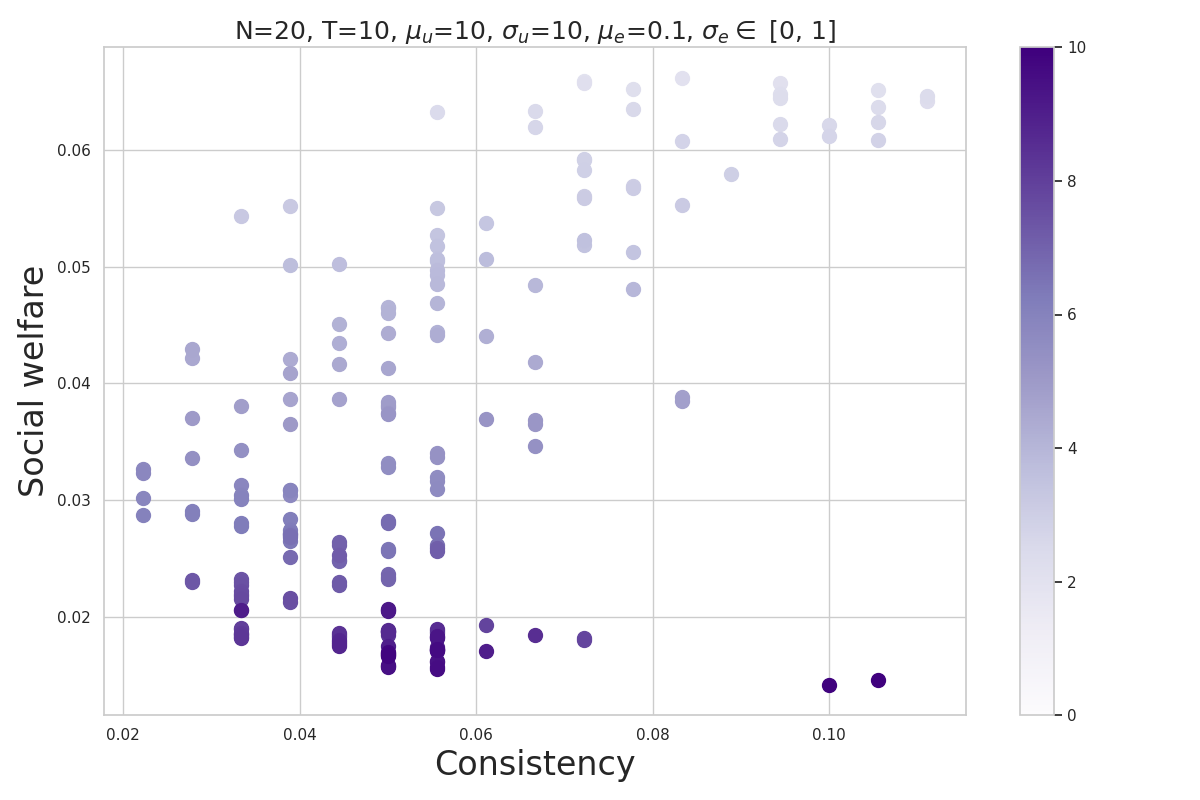
\includegraphics[width=\textwidth]{figures/mpda_dynamics_excitement_std.png}
         \caption{Dynamic Excitement}
         \label{fig:excite_std}
     \end{subfigure}
         \begin{subfigure}[b]{0.49\textwidth}
         \centering
         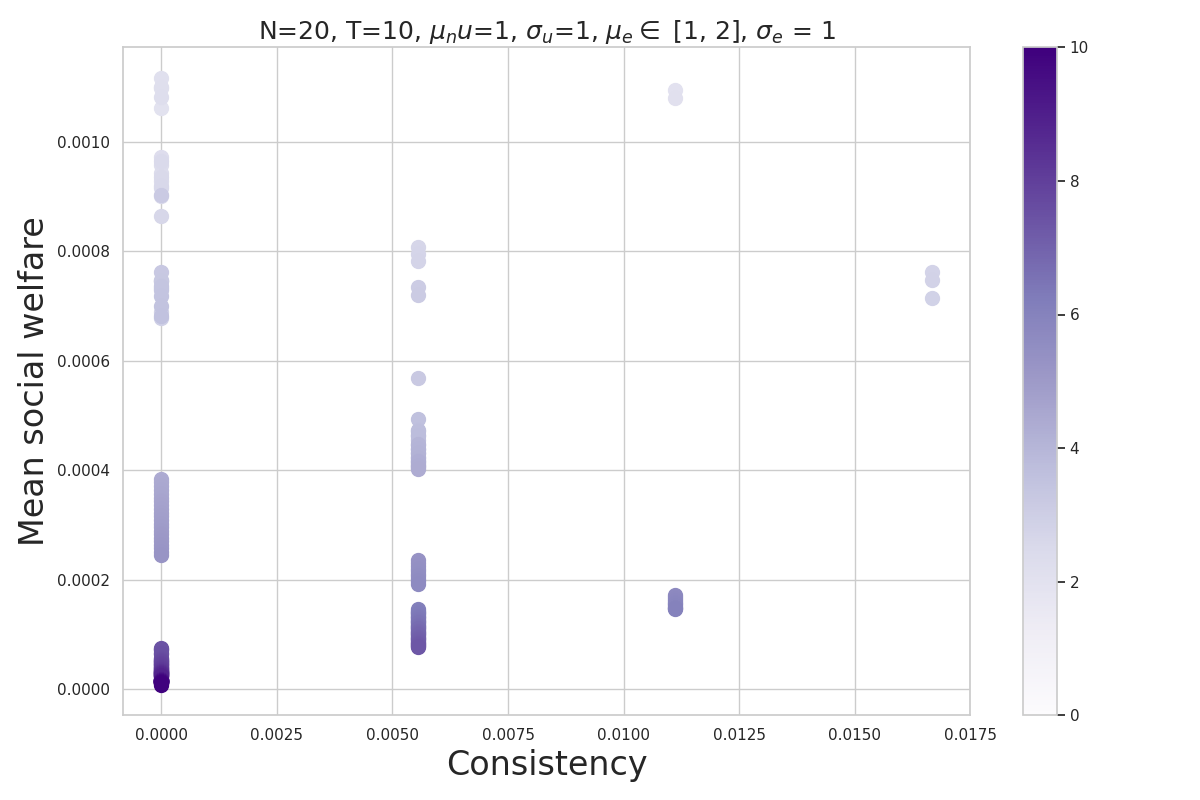
\includegraphics[width=\textwidth]{figures/mpda_dynamics_excitement_mean.png}
         \caption{Dynamic Excitement}
         \label{fig:excite_mean}
     \end{subfigure}
     \caption{Mean social welfare vs. consistency for MPDA applied to two dyanmic scenarios; (a) fixed excitement; (b) fixed initialization varying excitement (fixed mean); (c) fized initialization with varying excitement (fixed standard deviation).}
    \label{fig:mpda_dynamics}
\end{figure}